% A continuación se describen los participantes del modelo de negocio que influyen en la producción ganadera del CA-SENA-POP:

\section{Servicio Nacional de Aprendizaje (SENA)}

El SENA es un establecimiento público de educación en Colombia que ofrece formación gratuita con programas técnicos, tecnológicos y complementarios; que busca la incorporación y el desarrollo de las personas en actividades productivas que contribuyan al desarrollo social, económico y tecnológico del país. Entre las diferentes áreas de formación ofrecidas por el SENA, se encuentra el área de las ciencias agropecuarias, siendo esta la que tiene mayor influencia en la institución.\cite{sena}


\subsection{Centro Agropecuario}

El centro agropecuario (CA) tiene como objetivo liderar la formación de los sub-sectores agrícola, pecuario, pesquero y forestal de la región; mediante alianzas estratégicas con agremiaciones, administraciones municipales, campesinas y centros de educación técnica, media y superior. El CA incorpora tecnologías alternativas en las explotaciones agropecuarias para mejorar la calidad de los productos, reduciendo a su vez costos de producción. Dentro de los servicios ofertados por el CA-SENA se encuentran la producción y comercialización bovina y bufalina, procesamiento de alimentos y control de calidad (Cárnicos y Lácteos), entre otros\cite{casena}.

\section{Empresa donde se realiza el estudio: CA-SENA-POP}

El CA-SENA seccional Cauca, se encuentra ubicado en el norte de la ciudad de Popayán. Cuenta con una granja de aproximadamente 6 hectareas en las que realizan sus actividades productoras con unidades de producción bovina, porcina, avícola, bufalina, caprina, entre otras. Su formación y capacitación consta en gran medida de las prácticas realizadas por los aprendices en cada una de las unidades productoras.La granja se encuentra dividida en 2 zonas, el área usada para las instalaciones de la seccional Popayán y los lotes donde se realizan las diferentes prácticas y servicios mencionados con anterioridad.\\

Se cuenta con un total de 50 lotes de aproximadamente $500m^{2}$ cada uno (ver figura \ref{potrerosenapng}). 30 de ellos son usados para la producción silvopastoril bovina, 10 de ellos son usados para la producción de frutas, hierbas y hortalizas, entre ellas el botón de oro que es usado como forraje complementario en la dieta del ganado vacuno; y los lotes restantes son usados por las otras unidades productoras. Enfocándonos hacia la producción bovina, el CA-SENA-POP, se dedica a explotación del ganado vacuno con fines de producción lechera. Tal y como se ha mencionado antes, manejan un sistema de explotación silvopastoril semiestabulado, dado que distribuyen a sus animales en los diferentes lotes destinados para tal fin y llevan el registro de las cantidades de alimento concentrado y dietas secas, en un establo donde dosifican las cantidades correspondientes de sales minerales y proteínas concentradas.\\

\begin{figure}[H]
	 \begin{center}
	 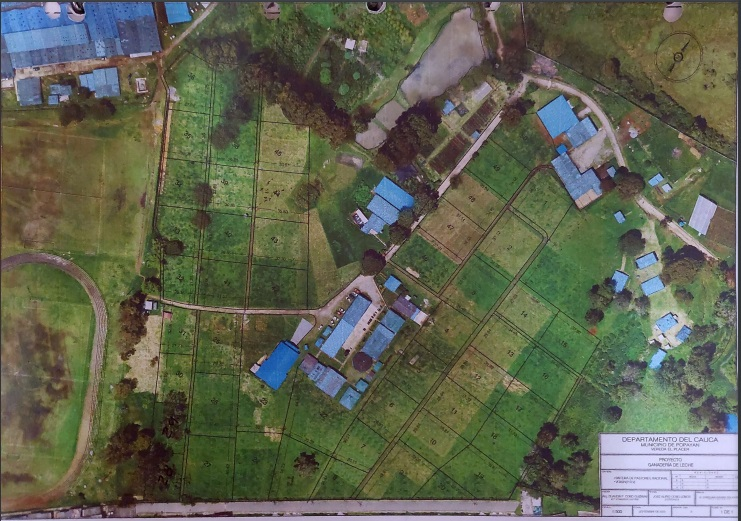
\includegraphics[scale=0.675]{img/potrerosena.jpg}
	 \end{center}
	 \caption{Granja del CA-SENA-POP. \label{potrerosenapng}}
	\end{figure}
	
\section{Negocio y comercialización de productos}

El CA-SENA-POP, realiza la venta de productos ganaderos entre los que se puede mencionar, la producción de leche cruda, reses productoras de leche y terneros para engorde. El CA-SENA-POP ha manifestado que los precios de compra y venta son los precios manejados en el mercado tanto por kg de peso del animal como por kilogramo de leche producida.\\


En el capítulo siguiente, se realiza una descripción de los datos presentes en el CA-SENA-POP usados para este proyecto de investigación


